En un procesador segmentado, varias instrucciones se encuentran en distintas
etapas al mismo tiempo. Esa superposición mejora el aprovechamiento del
pipeline, pero también exige coordinar instrucciones que comparten datos o que
pueden modificar el flujo de ejecución. En este capítulo se explican los
\emph{hazards} que aparecen en el diseño y los mecanismos que permiten resolverlos.

\section{Por qué aparecen hazards}

Una dependencia de datos aparece cuando una instrucción necesita el resultado
de otra que todavía está en el pipeline. Por ejemplo, una suma puede producir
un valor que la instrucción siguiente debe utilizar. Si esta última toma el
valor anterior del banco de registros, ejecuta la operación con un operando
incorrecto.

Para evitarlo, el procesador utiliza tres mecanismos según el momento en que el
resultado está disponible y la etapa que lo necesita:

\begin{itemize}
  \item \textbf{Forwarding hacia EX:} reenvía un resultado disponible desde
    \code{EX/MEM} o \code{MEM/WB} a la instrucción que lo necesita en EX.
  \item \textbf{Bypass \tech{WB}$\rightarrow$\tech{ID}:} entrega a ID el valor
    que WB está por escribir cuando ambas etapas acceden al mismo registro.
  \item \textbf{Espera \code{load-use}:} retrasa al consumidor inmediato de un
    load hasta que el dato leído de memoria está disponible para forwarding.
\end{itemize}

También pueden aparecer dependencias de control, por ejemplo cuando un branch
tomado cambia la dirección desde la que deben buscarse las instrucciones. La
tabla~\ref{tab:tipos-hazard} resume los casos considerados y cómo los trata el
diseño.

\begin{table}[H]
  \centering
  \small
  \begin{tabularx}{\textwidth}{L{3.0cm}L{3.6cm}Y}
    \toprule
    \textbf{Clase} & \textbf{Ejemplo} & \textbf{Tratamiento} \\
    \midrule
    Dato RAW & \code{add} seguido de un consumidor de su resultado &
    Forwarding desde \code{EX/MEM} o \code{MEM/WB}; bypass
    \tech{WB}$\rightarrow$\tech{ID} si el productor está en WB. \\
    \addlinespace
    Dato RAW con load & \code{lw} seguido de un consumidor inmediato &
    \code{load-use}: retener el consumidor e insertar una burbuja. \\
    \addlinespace
    Control & Branch tomado, \code{JAL} o \code{JALR} & Resolución en EX;
    redirect y descarte de las dos instrucciones jóvenes. \\
    \addlinespace
    Estructural & IF y MEM en el mismo ciclo & No existe: IMEM y DMEM son
    espacios independientes y permiten accesos simultáneos. \\
    \addlinespace
    WAW / WAR & Dos escrituras o una lectura y una escritura & No existen en un
    pipeline \emph{in-order} con escritura única en WB. \\
    \bottomrule
  \end{tabularx}
  \caption{Clases de hazard y su tratamiento.}
  \label{tab:tipos-hazard}
\end{table}

La especificación completa, con ecuaciones y prioridades, se encuentra en
\doc{architecture/cpu/control_and_hazards.md}{Control y hazards}.

\section{Forwarding hacia EX}

Cuando una instrucción llega a EX, los operandos que trajo desde ID pueden
haber quedado desactualizados: una instrucción anterior todavía puede tener el
resultado más reciente dentro del pipeline. El forwarding resuelve ese caso
sin esperar a que el resultado se escriba y vuelva a leerse del banco de
registros.

Para cada fuente que la instrucción utiliza, la unidad de forwarding compara
su número de registro con los destinos de las instrucciones que están en
\code{EX/MEM} y \code{MEM/WB}. Si encuentra un productor válido, selecciona
su resultado; en caso contrario, conserva el valor que llegó en \code{ID/EX}.

La comparación considera únicamente instrucciones válidas que escriben un
registro distinto de \code{x0}, y solo examina las fuentes que el consumidor
usa realmente. Si ambos registros interetapa contienen un productor del mismo
destino, se aplica la siguiente prioridad:

\begin{codebox}
EX/MEM > MEM/WB > valor base ID/EX
\end{codebox}

\code{EX/MEM} tiene prioridad porque contiene la instrucción productora más
reciente. La figura~\ref{fig:forwarding} muestra cómo los valores de ambos
registros interetapa llegan a los selectores de operandos de EX, junto con los
valores originales transportados por \code{ID/EX}.

\begin{figure}[H]
  \centering
  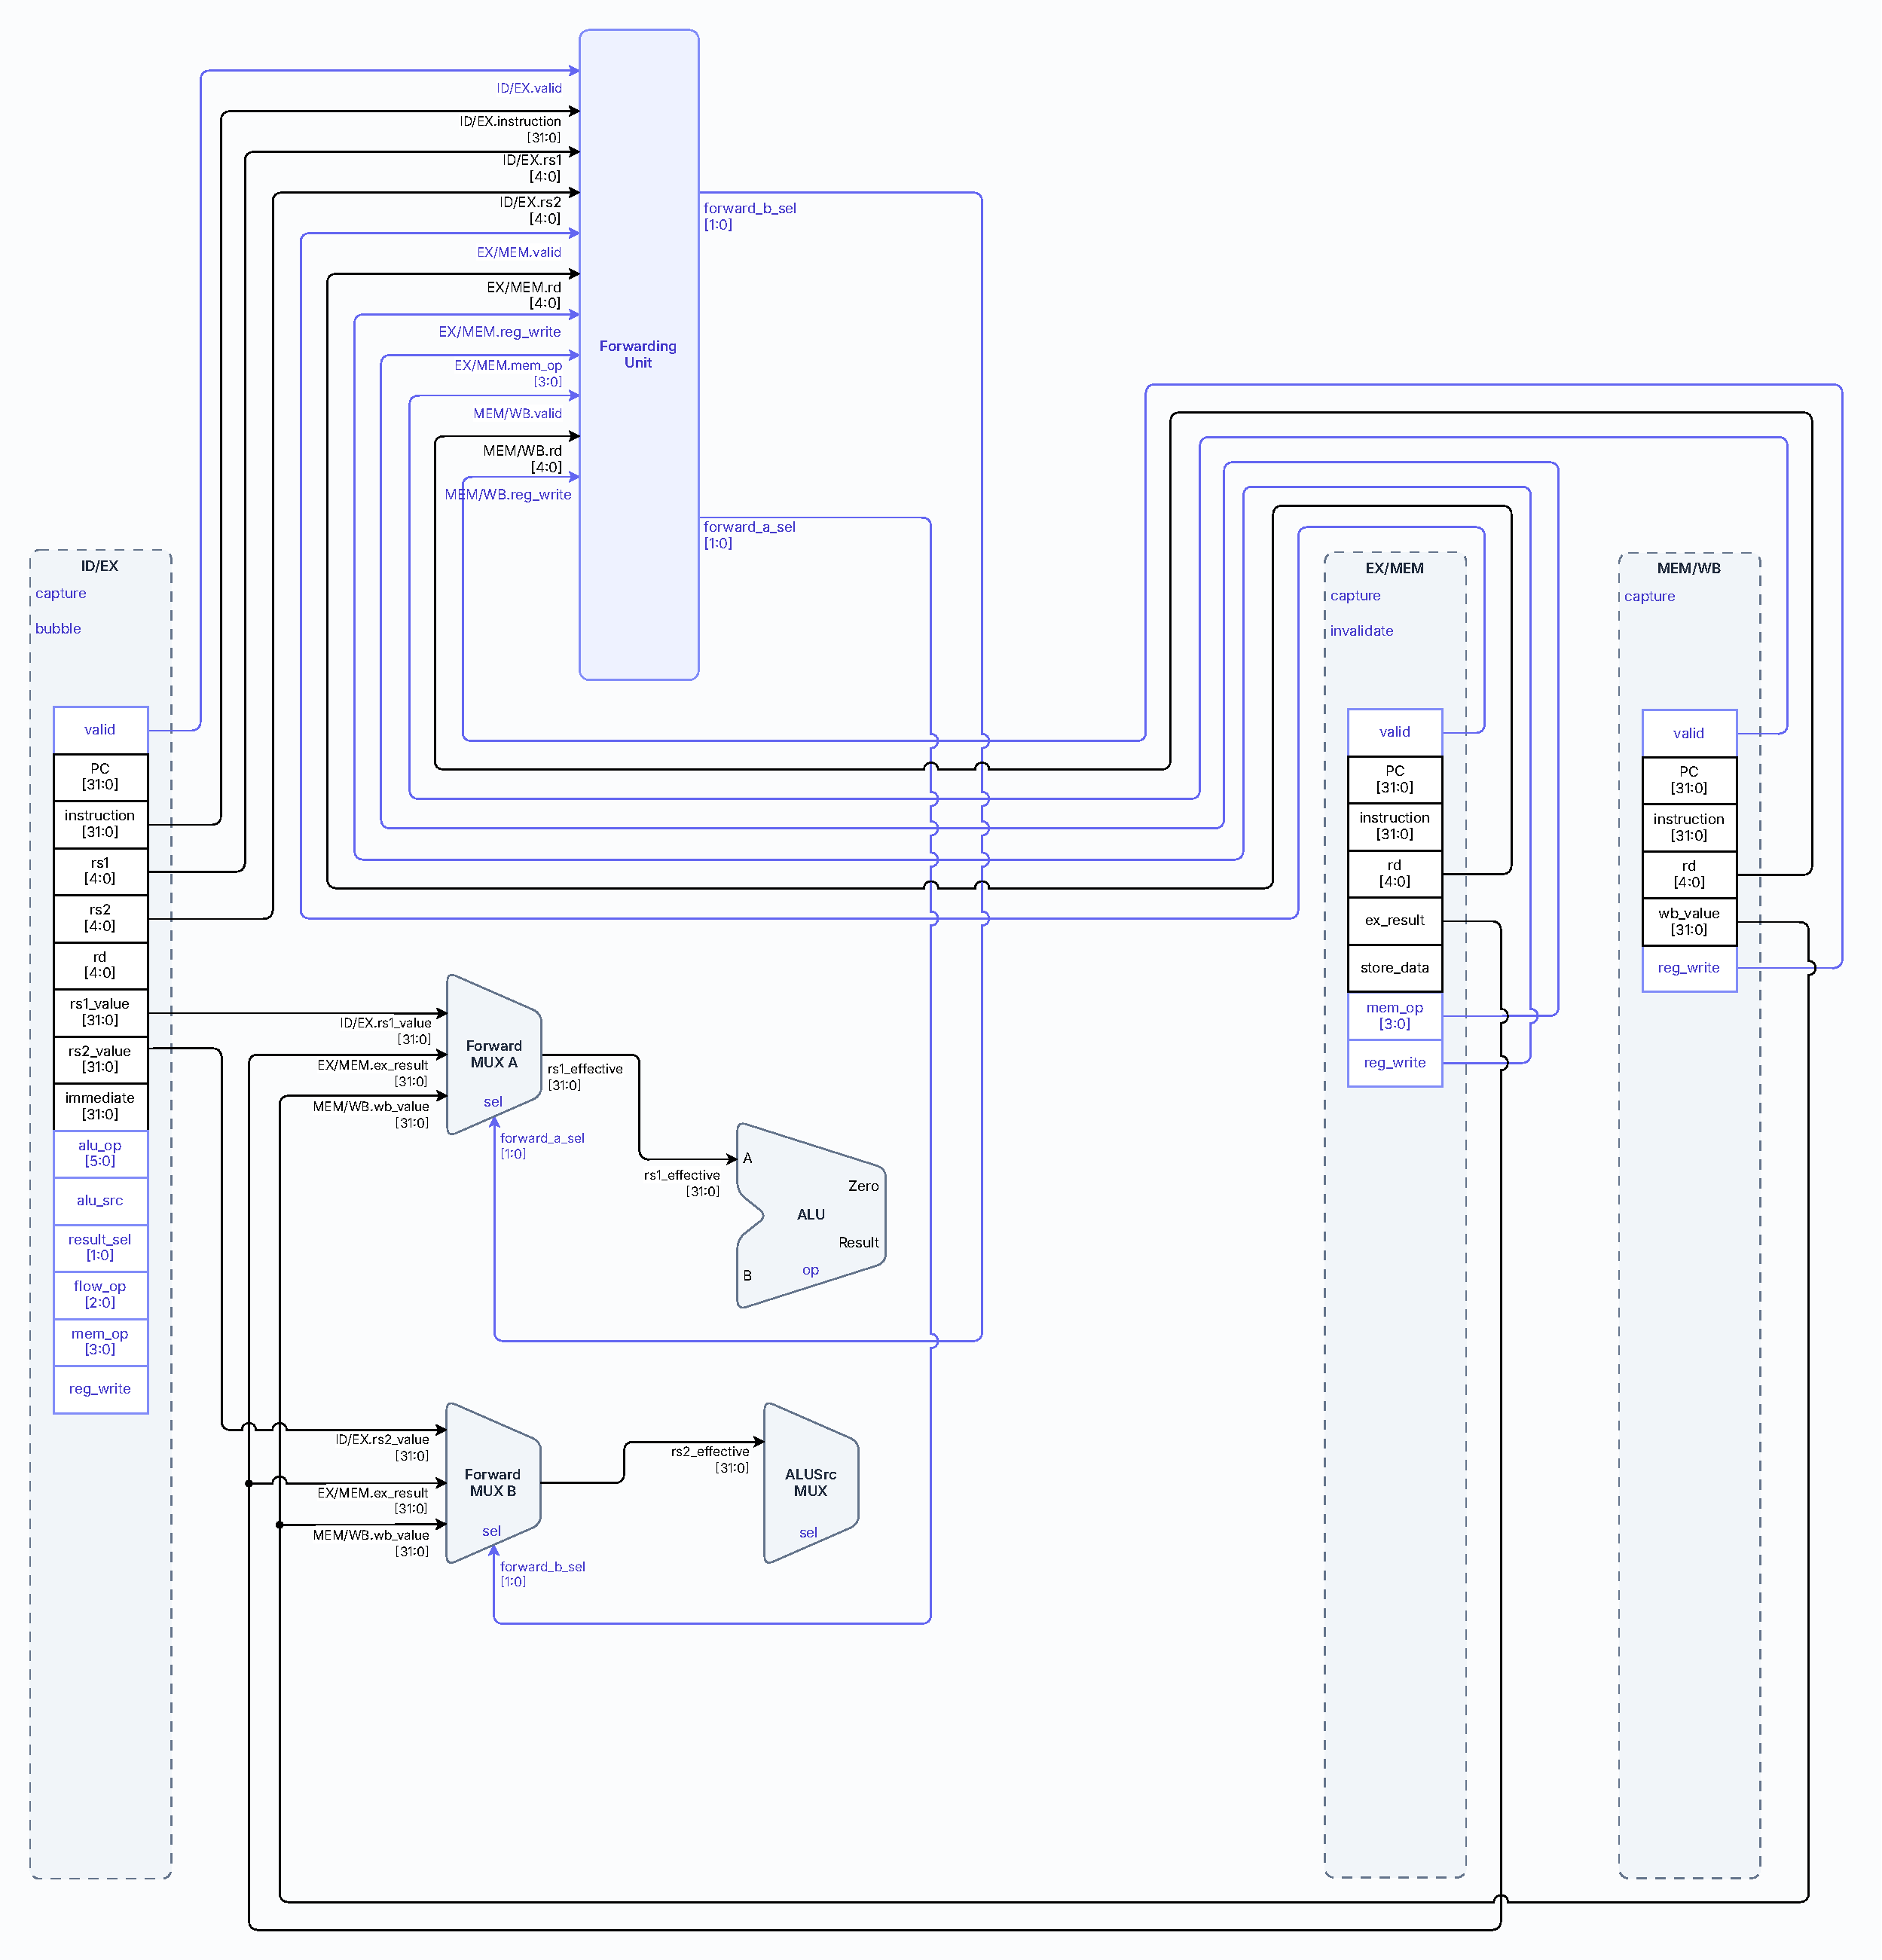
\includegraphics[width=0.95\textwidth,height=0.68\textheight,keepaspectratio]{forwarding.pdf}
  \caption{Recorrido del forwarding hacia los operandos de EX.}
  \label{fig:forwarding}
\end{figure}

\subsection{Ejemplo de forwarding desde \code{EX/MEM}}

Considérese la secuencia:

\begin{codebox}[language=RISCV]
add x1, x4, x5
sub x2, x1, x3
\end{codebox}

La tabla~\ref{tab:forwarding-exmem} muestra los ciclos relevantes. En C4, el
\code{add} está en MEM y el \code{sub} en EX; el resultado de \code{x1} todavía
no se escribió en el banco de registros, pero ya está en \code{EX/MEM}.
Forwarding selecciona ese valor y el \code{sub} opera con el dato correcto.

\begin{table}[H]
  \centering
  \small
  \begin{tabular}{clll}
    \toprule
    \textbf{Ciclo} & \textbf{\code{add}} & \textbf{\code{sub}} & \textbf{Acción} \\
    \midrule
    C3 & EX & ID & ID lee el valor base de \code{x1}. \\
    C4 & MEM & EX & Forwarding desde \code{EX/MEM} hacia la fuente 1. \\
    C5 & WB & MEM & WB escribe \code{x1}; el resultado de \code{sub} avanza. \\
    C6 & --- & WB & WB escribe \code{x2}. \\
    \bottomrule
  \end{tabular}
  \caption{Forwarding desde \code{EX/MEM} para el consumidor inmediato.}
  \label{tab:forwarding-exmem}
\end{table}

\subsection{El caso especial del load}

Un load requiere una consideración adicional. Al salir de EX, su resultado es
la dirección efectiva del acceso; el dato solicitado recién se obtiene en MEM.
Por lo tanto, la dirección que transporta \code{EX/MEM.ex_result} no puede
reenviarse como si fuera el valor que el load escribirá en el registro destino.

Si ese load es el productor más reciente, tampoco corresponde utilizar una
versión anterior del mismo registro desde \code{MEM/WB}. Las siguientes
condiciones expresan esa regla para cada fuente:

La condición de disponibilidad se expresa como:

\begin{codebox}
exmem_result_available = !is_load(EX/MEM.mem_op)
forward_exmem_rsN = exmem_match_rsN && exmem_result_available
forward_memwb_rsN = !exmem_match_rsN && memwb_match_rsN
\end{codebox}

La selección desde \code{MEM/WB} se bloquea cuando hay coincidencia con
\code{EX/MEM}, incluso si ese productor es un load cuyo dato aún no está
disponible. La espera \code{load-use}, explicada más adelante, evita que el
consumidor inmediato llegue a EX antes de tiempo.

\section{Bypass \texorpdfstring{WB$\rightarrow$ID}{WB a ID}}

El bypass entre WB e ID resuelve otra situación: una instrucción está por
escribir su resultado en el banco de registros mientras otra, en ID, lee ese
mismo registro. Como ambas operaciones coinciden en el ciclo, el valor leído
del banco podría no reflejar todavía la escritura.

Para que el consumidor reciba el resultado correcto, el bypass toma el valor
de WB y lo entrega directamente al puerto de lectura correspondiente. Así, el
comportamiento no depende del orden de lectura y escritura del banco en ese
flanco.

La selección se evalúa por separado para cada fuente y requiere que la escritura
de WB esté efectivamente habilitada:

\begin{codebox}
bypass_rs1 = rf_write_fire && (MEM/WB.rd == id_rs1)
bypass_rs2 = rf_write_fire && (MEM/WB.rd == id_rs2)
\end{codebox}

Cuando hay coincidencia, el puerto correspondiente selecciona
\code{MEM/WB.wb_value}; en caso contrario, conserva la lectura del banco. Los
valores seleccionados se capturan en \code{ID/EX} para que EX los utilice en el
ciclo siguiente. Si entonces existe un productor más reciente, el forwarding
de EX puede volver a reemplazarlos. La figura~\ref{fig:bypass} muestra estos
caminos desde WB y el banco de registros hasta los operandos de ID.

\begin{figure}[H]
  \centering
  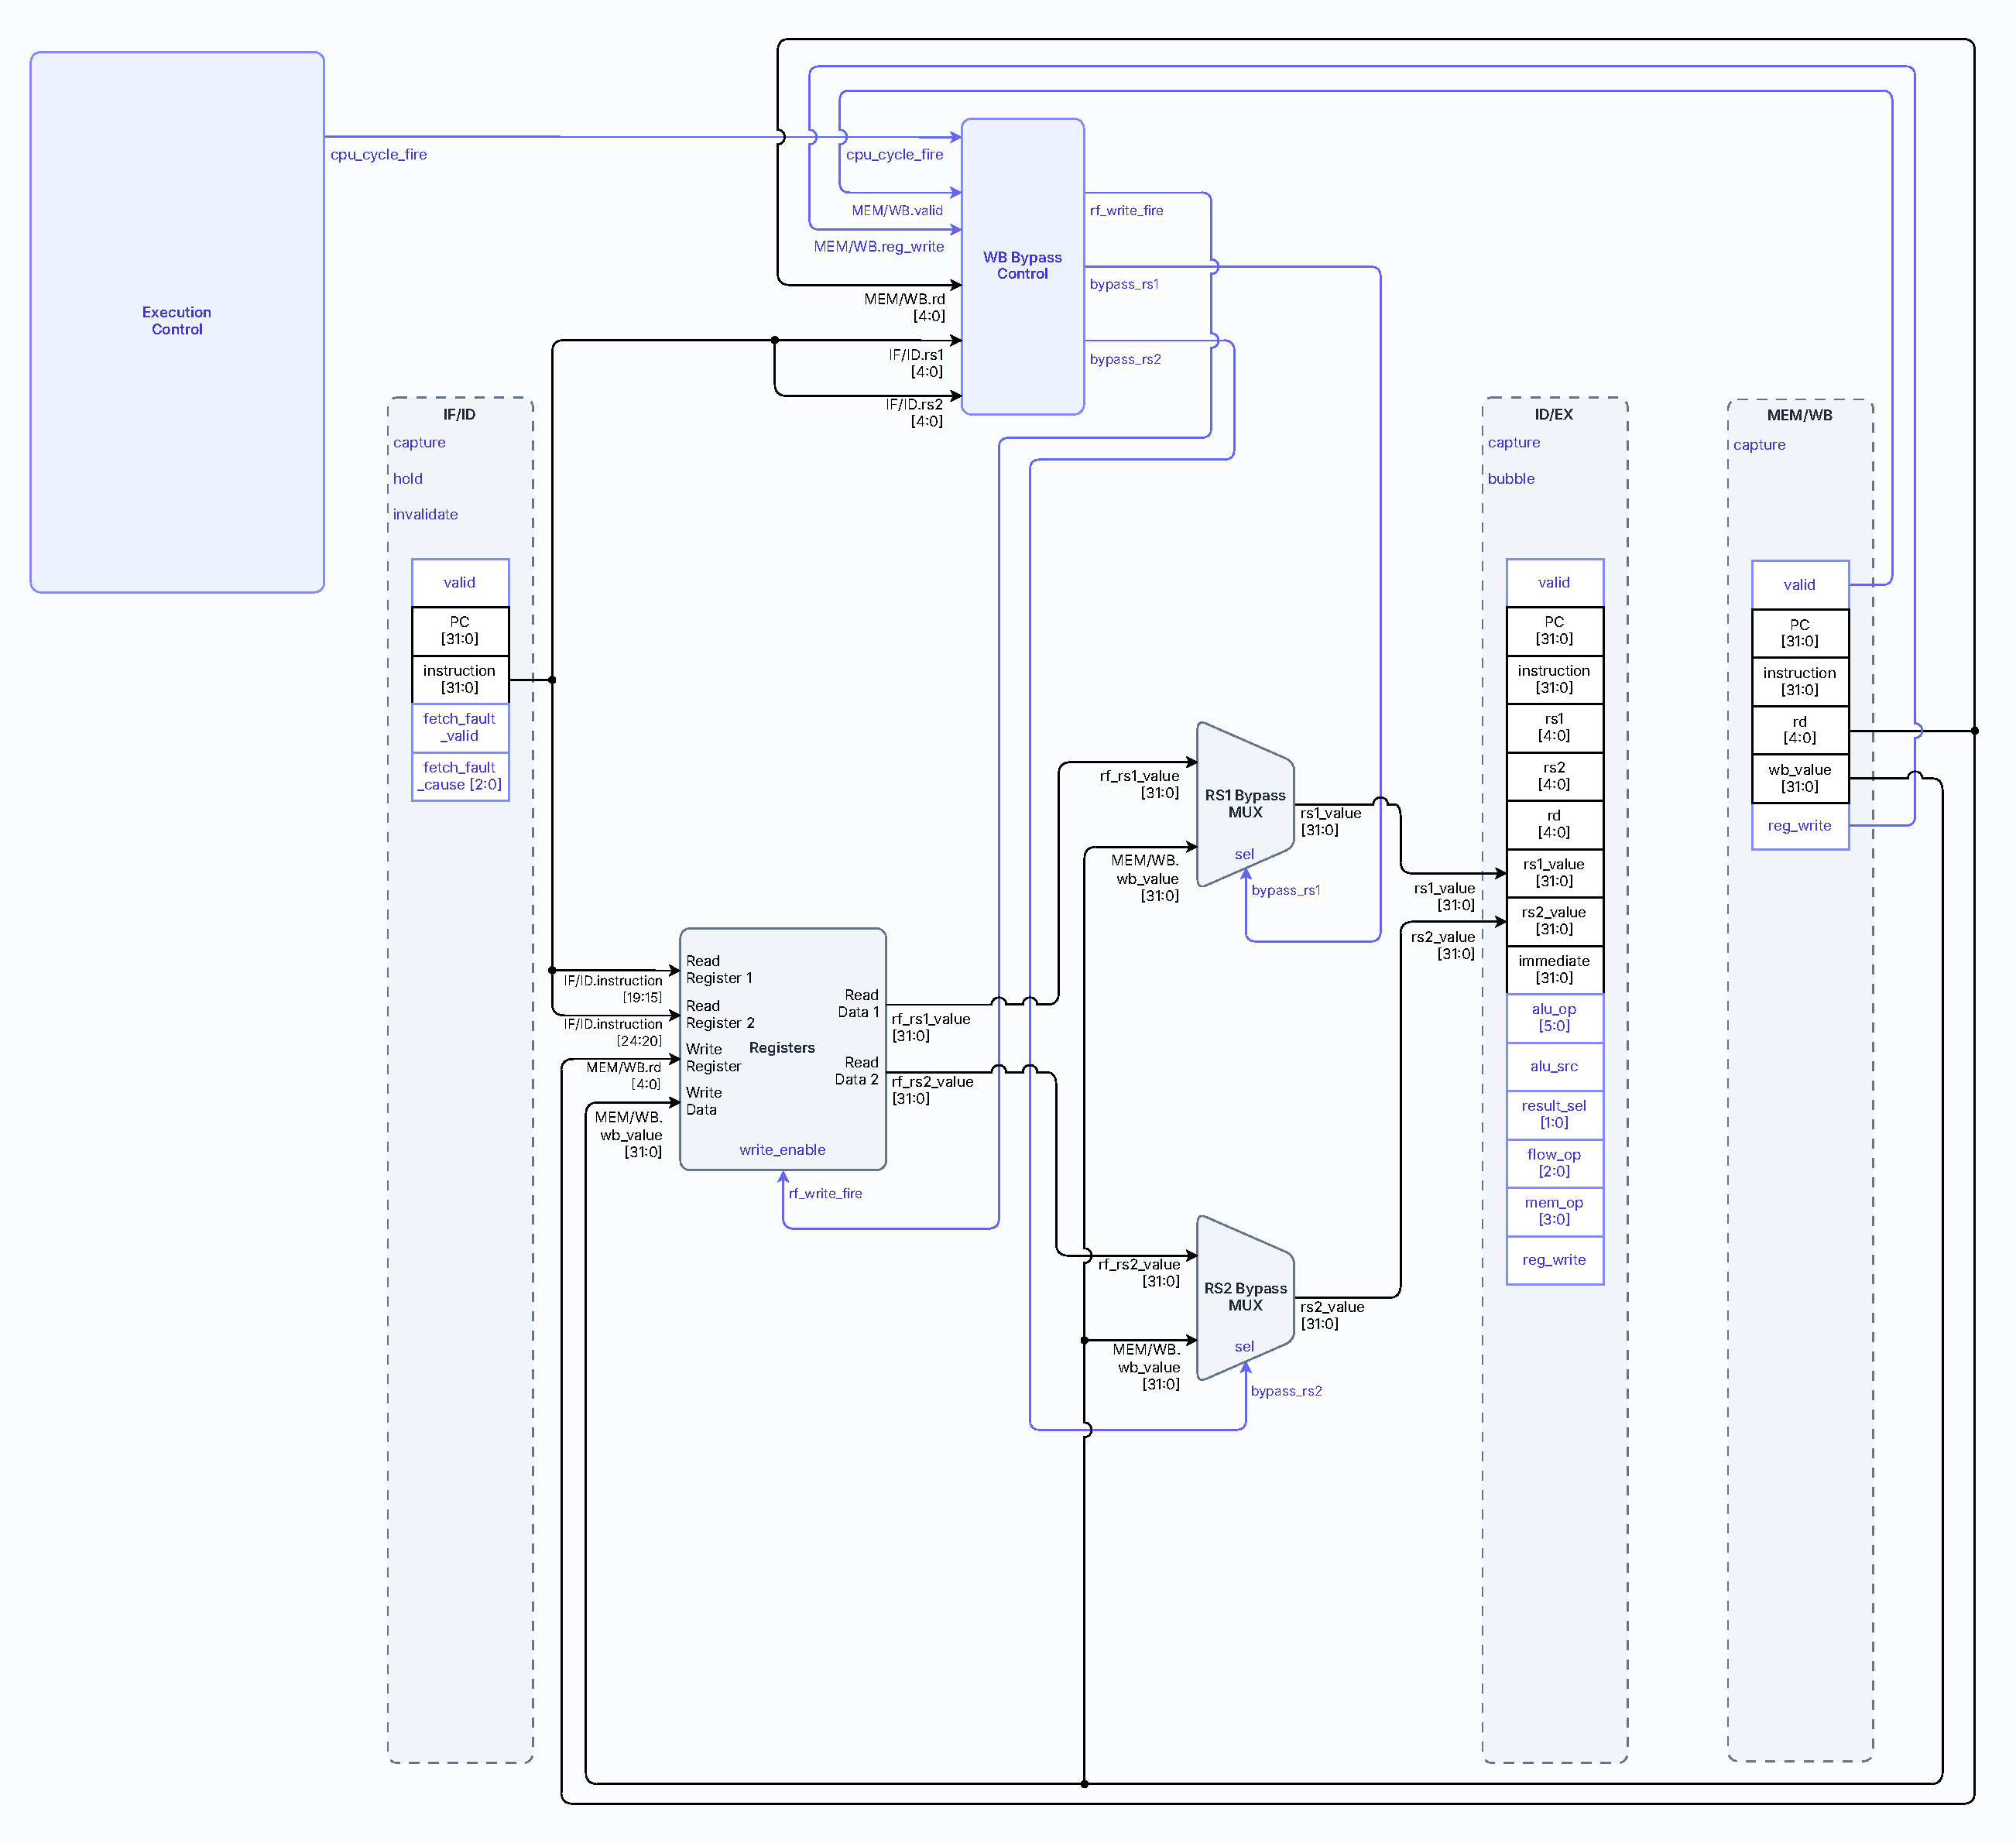
\includegraphics[width=0.95\textwidth,height=0.68\textheight,keepaspectratio]{bypass.pdf}
  \caption{Bypass \texorpdfstring{WB$\rightarrow$ID}{WB a ID}.}
  \label{fig:bypass}
\end{figure}

\section{Dependencia \texorpdfstring{load-use}{load-use}}

\subsection{Detección}

Una instrucción que utiliza inmediatamente el resultado de un load necesita una
espera. Cuando el load está en EX, calcula la dirección efectiva, pero el dato
se leerá en MEM durante el ciclo siguiente. Si ambas instrucciones avanzaran
sin demora, el consumidor llegaría a EX en ese mismo ciclo y necesitaría el
valor antes de que esté registrado en \code{MEM/WB}.

El diseño reenvía el resultado del load desde \code{MEM/WB}, por lo que retiene
al consumidor un ciclo para darle tiempo al load a completar la lectura.

Para reconocer esta dependencia, el detector compara el destino del load que
está en \code{ID/EX} con las fuentes utilizadas por la instrucción que espera
en \code{IF/ID}. La condición completa es:

\begin{codebox}
load_use_stall =
    ID/EX.valid
    && is_load(ID/EX.mem_op)
    && (ID/EX.rd != 0)
    && IF/ID.valid
    && (
         (ifid_uses_rs1 && (ifid_rs1 == ID/EX.rd))
         ||
         (ifid_uses_rs2 && (ifid_rs2 == ID/EX.rd))
       )
\end{codebox}

Una coincidencia accidental en un campo que la instrucción no usa no genera
dependencia. Tampoco participa un candidato de fetch, porque tiene
\code{IF/ID.valid = 0}. Un load con destino \code{x0} no crea dependencia.

\subsection{Efecto}

Cuando se selecciona la acción \code{act_load_use}, el control retiene la
instrucción consumidora e inserta una burbuja detrás del load. Las instrucciones
más antiguas continúan avanzando:

\begin{codebox}
PC       -> retener
IF/ID    -> retener
ID/EX    -> bubble
EX/MEM   -> capturar EX
MEM/WB   -> capturar MEM
\end{codebox}

Durante el stall, el load pasa de EX a MEM y el consumidor permanece en ID. En
el ciclo siguiente, el load completa la lectura y su resultado se captura en
\code{MEM/WB}, mientras el consumidor avanza a \code{ID/EX}. Un ciclo después,
el consumidor llega a EX y recibe por forwarding el dato ya registrado.

Aunque el consumidor permanezca detenido, el stall es un ciclo efectivo: el
contador aumenta, las instrucciones anteriores pueden completar sus efectos y,
en modo \code{STEP}, se consume una orden. En \code{HOLD}, en cambio, no se
autoriza un ciclo de CPU.

\section{Ejemplo ciclo a ciclo: \texorpdfstring{\code{TEST-PIPE-005/C001}}{TEST-PIPE-005/C001}}

El caso \code{TEST-PIPE-005/C001} del manifiesto ejecuta el siguiente programa
en \code{processor_top}:

\begin{codebox}[language=RISCV]
lw   x1, 0(x0)
add  x3, x1, x2
halt
\end{codebox}

El estado inicial prepara \code{x2 = 3} y \code{DMEM[0] = 8}. El resultado
esperado es \code{x1 = 8}, \code{x3 = 11}; el caso registra siete ciclos, un
stall, la escritura de \code{x1} en el ciclo 5, la de \code{x3} en el ciclo 7 y
la acción de load-use en el ciclo 3. La tabla~\ref{tab:load-use} muestra las
instrucciones presentes en cada etapa durante cada ciclo; a continuación se
explican las acciones que se producen al finalizar cada uno.

\begin{table}[H]
  \centering
  \small
  \begin{tabular}{lccccccc}
    \toprule
    \textbf{Ciclo} & \textbf{C1} & \textbf{C2} & \textbf{C3} & \textbf{C4} & \textbf{C5} & \textbf{C6} & \textbf{C7} \\
    \midrule
    \textbf{IF}  & \code{lw} & \code{add} & \code{halt} & \code{halt} & --- & --- & --- \\
    \textbf{ID}  & --- & \code{lw} & \code{add} & \code{add} & \code{halt} & --- & --- \\
    \textbf{EX}  & --- & --- & \code{lw} & Burbuja & \code{add} & \code{halt} & --- \\
    \textbf{MEM} & --- & --- & --- & \code{lw} & Burbuja & \code{add} & --- \\
    \textbf{WB}  & --- & --- & --- & --- & \code{lw} & --- & \code{add} \\
    \bottomrule
  \end{tabular}
  \caption{Recorrido del caso \code{TEST-PIPE-005/C001} por ciclo y por etapa.
  Cada columna muestra el estado durante el ciclo, antes del flanco que lo cierra.}
  \label{tab:load-use}
\end{table}

El recorrido se desarrolla de la siguiente manera:

\begin{description}
  \item[C1:] Se busca \code{lw}, se captura en \code{IF/ID} y el PC pasa a 4.
  \item[C2:] Se busca \code{add}, el \code{lw} avanza a EX y el PC pasa a 8.
  \item[C3:] Se detecta la dependencia mientras \code{lw} está en EX y
    \code{add} en ID. En el flanco que cierra el ciclo se retienen el PC y
    \code{IF/ID}, \code{lw} avanza a \code{EX/MEM} y se invalida
    \code{ID/EX}, insertando la burbuja.
  \item[C4:] La burbuja ocupa EX, mientras \code{lw} está en MEM y
    \code{add} sigue en ID. Al cerrar el ciclo se captura \code{halt},
    \code{add} avanza a EX y el dato leído por \code{lw} se captura en
    \code{MEM/WB}.
  \item[C5:] El forwarding entrega ese dato al \code{add}, que calcula
    \code{x3 = 11}, mientras WB escribe \code{x1 = 8}.
  \item[C6:] Se confirma \code{halt} en EX, se descarta el trabajo posterior y el
    \code{add} avanza hacia WB.
  \item[C7:] WB escribe \code{x3 = 11}; el pipeline queda vacío y la sesión pasa a
    \code{FINISHED}.
\end{description}

\section{Cambios de flujo y descarte}

\subsection{Saltos y branches}

El procesador busca instrucciones de manera secuencial mientras las anteriores
avanzan por el pipeline. Sin embargo, un branch tomado o un salto puede indicar
que la ejecución debe continuar en otra dirección. Como esa decisión se toma
en EX, para entonces ya pueden haberse buscado dos instrucciones posteriores:
una está en ID y la otra en IF.

Cuando se confirma el cambio de flujo, también llamado \emph{redirect}, el PC
recibe la dirección de destino y se descartan esas dos instrucciones, porque
pertenecen al camino que se abandonó. La instrucción que produjo el cambio y
las anteriores continúan avanzando. En \code{JAL} y \code{JALR}, esto permite
conservar el valor de enlace que luego se escribirá en el registro destino.

El descarte de las dos instrucciones produce una penalización de dos ciclos.
La ejecución continúa desde el nuevo PC y mantiene la modalidad elegida:
\code{RUN} sigue avanzando automáticamente, mientras que \code{STEP} espera la
siguiente orden.

\subsection{Faults y \code{halt}}

Cuando se confirma un fault o un \code{halt}, el procesador deja de admitir
instrucciones nuevas y descarta las que son posteriores al evento. Las
instrucciones anteriores, en cambio, pueden terminar sus efectos mediante el
drenado explicado en el capítulo anterior.

Si el fault se confirma en ID, la instrucción que está en EX es anterior y
puede avanzar. Si se confirma en EX, la instrucción que lo produjo se descarta
antes de llegar a MEM. Por su parte, \code{halt} se consume en EX y representa
una terminación normal.

\subsection{Selección de la acción del pipeline}

En cada ciclo efectivo, \code{Pipeline Hazard Control} decide cómo actualizar
el PC y los registros entre etapas. Por ejemplo, ante una dependencia
\code{load-use} retiene al consumidor, mientras que ante un redirect descarta
las instrucciones del camino anterior. La tabla~\ref{tab:acciones} resume
estas decisiones, incluidas las que se utilizan durante el drenado.

En la tabla, «Capt.» indica que el registro recibe la salida de la etapa
señalada y «Burbuja» representa una entrada inválida. Al invalidar \code{IF/ID}
se limpian tanto \code{valid} como \code{fetch_fault_valid}; en los demás
registros, la invalidez se indica con \code{valid=0}.

\begin{table}[H]
  \centering
  \footnotesize
  \setlength{\tabcolsep}{3pt}
  \begin{tabularx}{\textwidth}{L{3.75cm}ZZZZZ}
    \toprule
    \textbf{Acción} & \textbf{PC} & \textbf{IF/ID} & \textbf{ID/EX} &
    \textbf{EX/MEM} & \textbf{MEM/WB} \\
    \midrule
    Fault en EX & Retener & Invalidar & Burbuja & Invalidar & Capt. MEM \\
    \code{halt} en EX & Retener & Invalidar & Burbuja & Invalidar & Capt. MEM \\
    Redirect & Destino & Invalidar & Burbuja & Capt. EX & Capt. MEM \\
    Fault en ID & Retener & Invalidar & Burbuja & Capt. EX & Capt. MEM \\
    \code{load-use} & Retener & Retener & Burbuja & Capt. EX & Capt. MEM \\
    Avance normal & PC+4 & Capt. IF & Capt. ID & Capt. EX & Capt. MEM \\
    Drenado con \code{load-use} & Retener & Retener & Burbuja & Capt. EX & Capt. MEM \\
    Avance de drenado & Retener & Invalidar & Capt. ID & Capt. EX & Capt. MEM \\
    \bottomrule
  \end{tabularx}
  \caption{Efecto de las acciones sobre el PC y los registros interetapa.}
  \label{tab:acciones}
\end{table}

Si varios eventos ocurren en el mismo ciclo, se selecciona una sola acción. En
ejecución ordinaria, el control los considera en este orden:

\begin{enumerate}
  \item fault de la instrucción en EX;
  \item \code{halt} en EX;
  \item redirect resuelto en EX;
  \item fault de la instrucción en ID;
  \item dependencia \code{load-use}.
\end{enumerate}

Si no ocurre ninguno de ellos, el pipeline avanza normalmente. Este orden
permite atender primero los eventos de la instrucción más antigua: la que está
en EX precede en el programa a la que está en ID. Durante el drenado se
seleccionan las acciones propias de esa fase; la variante de drenado con
\code{load-use} se conserva en el control, aunque no aparece en un drenado
legal. Las condiciones completas se detallan en
\doc{architecture/cpu/control_and_hazards.md}{Control y hazards}.
